%\exer{Application: déplacement d'un cavalier sur un échiquier}
%\vspace{-0.5cm}
\section*{Exercice d'application}

Soit les graphes suivants appelés \lstinline{poly}, \lstinline{maison}, \lstinline{foo1} et \lstinline{foo2}.
\begin{figure}[H]
	%\begin{center}
		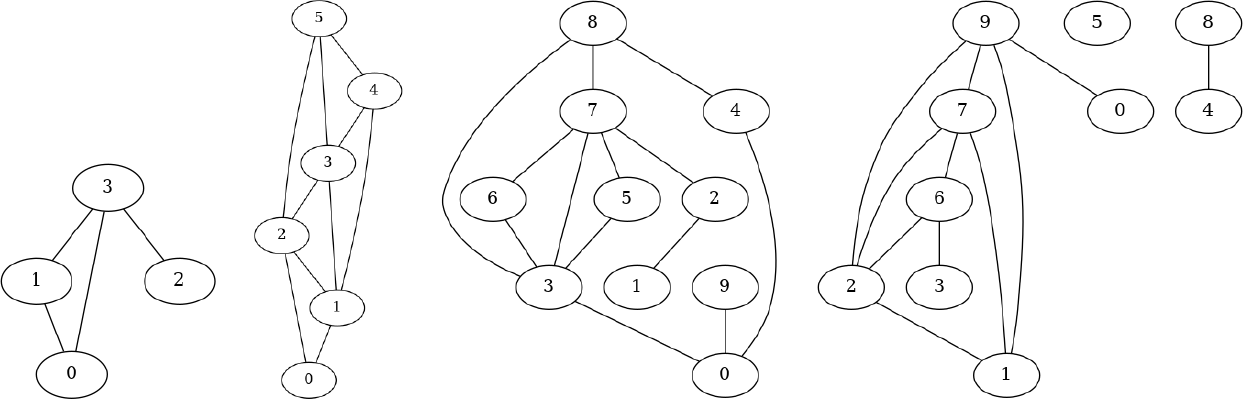
\includegraphics[width=\linewidth]{images/figure_01}
	%\end{center}
	\caption{ \lstinline{poly}, \lstinline{maison}, \lstinline{foo1} et \lstinline{foo2}}
\end{figure}

\question{Donner la représentation sous forme de dictionnaire d'adjacence de chacun de ces graphes.}


Un graphe connexe est déclaré :
\begin{itemize}
\item \textbf{semi-eulérien} lorsqu’il possède un chemin passant exactement une fois par chaque arête ;
\item \textbf{eulérien} lorsqu’il possède un cycle (le sommet de départ est celui d’arrivée) passant exactement
une fois par chaque arête ;
\item \textbf{hamiltonien} lorsqu’il possède un cycle passant exactement une fois par tous les sommets (sauf
celui de départ qui est celui d’arrivée).
\end{itemize}

\question{Parmi les graphes ci-dessus, en observer quelques-uns, et dire s’ils sont (semi-)eulériens et/ou hamiltoniens.}

Il est remarquable que ces propriétés qui se ressemblent en première approximation sont en fait de
complexité très différente à vérifier :
\begin{itemize}
\item un graphe est eulérien si, et seulement si, tous ses sommets sont de degré pair (le degré est le
nombre d’arêtes issues de ce sommet) ;
\item un graphe est semi-eulérien si, et seulement si, tous ses sommets sauf au plus 2 sont de degré
pair ;
\item pour tester le caractère hamiltonien, on ne sait pas faire bien mieux que de tester tous les
chemins possibles, ce qui en fait beaucoup ! %(Mais si vous avez une idée qui marche, venez m’en
%parler discrètement).
\end{itemize}

\marginnote{Attention. Le critère pour les (semi-)eulériens est « un petit peu faux ».}
% Je vous laisse le mettre en défaut.

\question{Écrire un programme testant le caractère eulérien ou semi-eulérien d’un graphe.}

Pour le caractère hamiltonien, on peut tenter de tester toutes les permutations possibles des sommets.
On dispose d’une fonction permettant d’engendrer toutes les permutations d’une liste !

\begin{lstlisting}
>>> from itertools import permutations
>>> for p in permutations(list(range(3))):
            print(p, list(p), list(p)+[p[0]])
                (0, 1, 2) [0, 1, 2] [0, 1, 2, 0]
                (0, 2, 1) [0, 2, 1] [0, 2, 1, 0]
                (1, 0, 2) [1, 0, 2] [1, 0, 2, 1]
                (1, 2, 0) [1, 2, 0] [1, 2, 0, 1]
                (2, 0, 1) [2, 0, 1] [2, 0, 1, 2]
                (2, 1, 0) [2, 1, 0] [2, 1, 0, 2]
\end{lstlisting}

Ainsi, on peut parcourir toutes les permutations ; pour chacune d’entre-elles, on ajoute le sommet
de départ à la fin, et on teste la présence dans les arêtes de toutes les jonctions $\left(s_{\sigma(i)},s_{\sigma(i+1)} \right)$.


\question{Écrire une fonction chemin testant si un chemin est présent dans
un graphe. Écrire ensuite une fonction testant le caractère hamiltonien d’un graphe.}

On peut voir sur ces tests que doit rendre la fonction lorsque le graphe est hamiltonien, un chemin le prouvant :

\begin{lstlisting}
>>> chemin([0, 1, 2, 3], maison)
    True
>>> chemin([0, 1, 2, 4], maison)
    False
>>> hamiltonien(maison)
    (True, [0, 1, 3, 4, 5, 2, 0])
>>> hamiltonien(poly)
    False
\end{lstlisting}


%\question{Qu’est-ce qui semble plus accessible : tester le caractère hamiltonien
%de cent graphes à dix sommets, ou bien mille graphes à cinq sommets ?}

%\begin{lstlisting}
%cpt = 0
%for i in range(100):
%    foo = lecture_graphe_mat("graphes-fournis/exemples5_%i.gr" % i)
%    if hamiltonien(foo): # le test est validé dès que le résultat n'est pas False :-)
%        cpt += 1
%        print("Il y a %i graphes à 5 sommets hamiltoniens" % cpt)
%\end{lstlisting}
%Il y a 4 graphes à 5 sommets hamiltoniens.